\documentclass[14pt]{extarticle}
\usepackage{amsmath}
\usepackage{amssymb}
\usepackage{graphicx}
\usepackage{tikz}
\usetikzlibrary{trees}
\usepackage{graphicx}
\graphicspath{ {../chap04/} }
\usepackage[top=0.75in, bottom=0.75in, left=0.75in, right=0.75in]{geometry}
\newcommand*{\Scale}[2][4]{\scalebox{#1}{\ensuremath{#2}}}%
\usepackage[shortlabels]{enumitem}
% \usepackage{showframe}
\title{\vspace{-5ex}Math 208 Sections 4.1 and 4.2}
\date{\vspace{-10ex}}
\usepackage{multicol}
\setlength{\columnsep}{1cm}

\begin{document}
\maketitle		
\section{Homework and other}
\begin{itemize}
\item Sections 3.2, 3.2
\item Sections 4.1, 4.2
\item Section 4.3
\end{itemize}

\section{Goals}
\begin{itemize}
	\item Review problem areas from the quiz
	\item Understand and apply solutions for a System of Linear Equations 
	\begin{enumerate}[(i)]
		\item Graphical,
		\item Substitution, and
		\item Elimination by Addition.
	\end{enumerate}
	\item Describe and understand the basics of a matrix.
	\item Convert a System of Linear Equations into an augmented matrix.
	\item State the allowable elementary row operations
	\item Analyze reduced matrix forms for solution types
\end{itemize}

\section{Quiz 1}
Please grade yourself on this quiz.
\begin{itemize}
	\item Mistakes on question 1-6? Review Section A.1 of the book, pages 872-876.
	\item Mistakes on questions 7-12? Review Section A.2 of the book, pages 879-882.
\end{itemize}

\section*{4.1 Systems of Linear Equations}
A \textit{linear equation} is an equation of the form $y=mx+b$. A System of Linear Equations is a set of such equations that must be solved simultaneously. In this section we deal only with two variable, two equation systems.
\begin{align*}
	ax+by &=h \\
	cx+dy &=k
\end{align*}
\subsection*{Graphical Method}
Given a system of equations, graph each line to determine the solution. Recall how to graph a line? Usually, this is most easily done by finding two points on each line.
\subsubsection*{Example}
\begin{itemize}
\item \textbf{Problem 15}:
\begin{align*}
	m+2n &= 4 \tag{a}\\
	2m + 4n &= -8 \tag{b}
\end{align*}
For (a); set $m=0$, then $n=2$ and set $n=0$, then $m=4$.\\
For (b); set $m=0$, then $n=-2$ and set $n=0$, then $m=-4$. \\
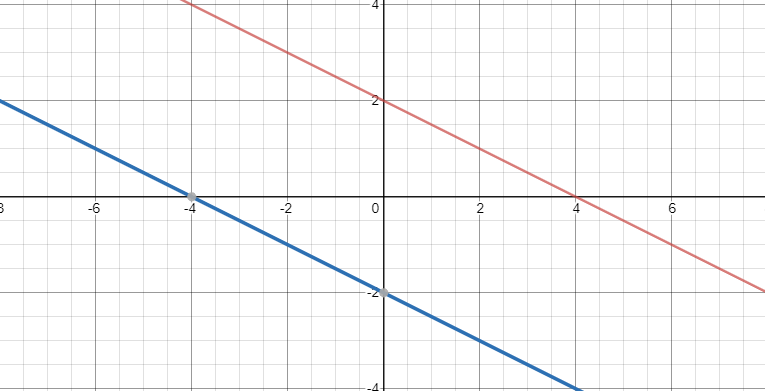
\includegraphics[width=0.85\linewidth]{4-1_a-15} \\
This is a graph of parallel lines. There is no intersection point therefore there exists \textbf{no solution}.
\subsubsection*{Solution types}
There are three types of solutions.
\begin{itemize}
	\item \textbf{No Solution} as graphed above with parallel lines. (\textbf{inconsistent})
	\item \textbf{One Solution} where the lines intersect. (\textbf{consistent and independent})
	\begin{align*}
		m+2n &= 4 \tag{a}\\
		2m + -4n &= -8 \tag{c}
	\end{align*}
	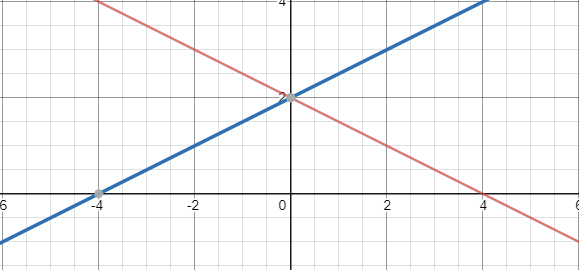
\includegraphics[width=0.45\linewidth]{4-1_a-15b}
	\item \textbf{Infinite Solutions} where the lines are the same line. (\textbf{consistent and dependent})
	\begin{align*}
		m+2n &= 4 \tag{a}\\
		-2m + 4n &= -8 \tag{d}
	\end{align*}
	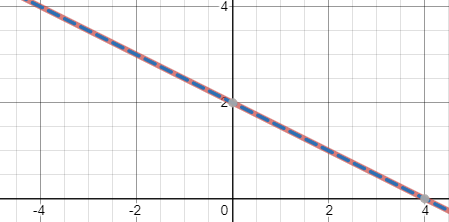
\includegraphics[width=0.45\linewidth]{4-1_a-15c}
\end{itemize}
\end{itemize}

\subsection*{Substitution Method}
This is probably the method you are most familiar with and works well for system with only two variables. We won't use this method other than in this chapter. We'll solve the system in problem 15 using substitution.
\subsubsection*{Example}
\begin{itemize}
	\item \textbf{Problem 15}:
	\begin{align*}
		m+2n &= 4 \tag{a}\\
		2m + 4n &= -8 \tag{b}
	\end{align*}
	Solve (a) for $m$, then $m= 4- 2n$. Now substitute this into (b).
	\begin{align*}
		2(4- 2n) + 4n &= -8 \\
		8-4n +4n &= -8 \\
		8 &= -8
	\end{align*}
	The result, $8=-8$, is a contradiction. This informs that there is no solution.
\end{itemize}

\subsection*{Elimination by Addition Method}
Another method you have learned in algebra. This method is more easily extended to systems of more than 2 variables and equations. In Elimination by Addition you may:
\begin{itemize}
	\item Interchange any two equations
	\item Multiply any equation by a non-zero constant
	\item Add a constant multiple of one equation to another equation
\end{itemize}
These same basic rules will be used in the next sextion when we begin using matrices to solve these systems.

\subsubsection*{Example}
\begin{itemize}
	\item \textbf{Problem 15}:
	\begin{align*}
		m+2n &= 4 \tag{a}\\
		2m + 4n &= -8 \tag{b}
	\end{align*}
	Add $-2 \times (a)$ to (b).
	\begin{align*}
		-2m -4n = -8& \\
		\underline{2m + 4n = -8}& \\
		0m+0n = -16&
	\end{align*}
	The result is a contradiction. This informs that there is no solution.
\end{itemize}

\cleardoublepage

\section*{4.2 Systems of Linear Equations and Augmented Matrices}
A \textit{matrix } is a rectangular array of values written inside of brackets. It has a size dimension denoted by $n \times m$ where $n$ is the number of rows and $m$ is the number of columns. The elements of a matrix are denoted by $a_{ij}$ where $i$ is the row and $j$ is the column the element is in. Some examples:
\\\\
A four element row matrix
\begin{align*}
	A = \begin{bmatrix}
		a_1 & a_2 & a_3 & a_4
	\end{bmatrix}
\end{align*}
A three element column matrix
\begin{align*}
	B = \begin{bmatrix}
		b_1 \\
		b_2 \\
		b_3
	\end{bmatrix}
\end{align*}
A general $3 \times 4$ matrix which has 12 elements.
\begin{align*}
	C = \begin{bmatrix}
		c_{1 1} & c_{1 2} & c_{1 3} & c_{1 4} \\
		c_{2 1} & c_{2 2} & c_{2 3} & c_{2 4} \\
		c_{3 1} & c_{3 2} & c_{3 3} & c_{3 4}
	\end{bmatrix}
\end{align*}
Notice that the matrix is indicated by an uppercase letter while its elements are indicated with lowercase letters.

\subsection*{Augmented Matrix}
An augmented matrix converts a system of linear equations to a matrix form to more easily and consistently solve it. Consider the system given in Problem 57:
\begin{align*}
	x_1 - 4x_2 &= -2 \\
	-2x_1 + x_2 &= -3
\end{align*}
We build a coefficient matrix and a constant matrix and then smash them together to create our augmented matrix.
\begin{align*}
	&\text{Coefficient Matrix} &\text{Constant Matrix} & \to &\text{Augmented Matrix} \\
	&\begin{bmatrix}
		-1 & -4 \\
		-2 & 1
	\end{bmatrix} 
	&\begin{bmatrix}
		-2 \\
		-3
	\end{bmatrix}
	& \to &\begin{bmatrix}
		-1 & -4 & | & -2\\
		-2 & 1 & | & -3
	\end{bmatrix}
\end{align*}

\subsection*{Row Operations}
Just as with the elimination by additional method, there are three row operations that are allowed. These operations produce row-equivalent matrices.
\begin{itemize}
	\item Interchange any two rows
	\item Multiply any row by a non-zero constant
	\item Add a constant multiple of one row to another
\end{itemize}
We use these operations to reduce the matrix to a reduced form of:
\begin{align*}
	\begin{bmatrix}
		1 & 0 & | & h \\
		0 & 1 & | & k
	\end{bmatrix}
\end{align*}
From this reduced form, the solution is readily found.

\subsubsection*{Example: Problem 57}
\begin{align*}
	x_1 - 4x_2 &= -2 \\
	-2x_1 + x_2 &= -3
\end{align*}
Convert to augmented matrix
\begin{align*}
	\begin{bmatrix}
		-1 & -4 & | & -2\\
		-2 & 1 & | & -3
	\end{bmatrix} \\
	&\to 
	\begin{array}{r}
		(-1)R1 \\
		R2
	\end{array}
	\begin{bmatrix}
		1 & 4 & | & 2\\
		-2 & 1 & | & -3
	\end{bmatrix} \\
	&\to 
	\begin{array}{r}
		R1 \\
		2R1+R2
	\end{array}
	\begin{bmatrix}
		1 & 4 & | & 2\\
		0 & 9 & | & 1
	\end{bmatrix} \\
	&\to 
	\begin{array}{r}
		R1 \\
		(1/9)R2
	\end{array}
	\begin{bmatrix}
		1 & 4 & | & 2\\
		0 & 1 & | & 1/9
	\end{bmatrix} \\
	&\to 
	\begin{array}{r}
		-4R2 + R1 \\
		R2
	\end{array}
	\begin{bmatrix}
		1 & 0 & | & 14/9\\
		0 & 1 & | & 1/9
	\end{bmatrix} \\
\end{align*}
From this result, we determine that $x_1=14/9$ and $x_2 = 1/9$. The details of the method we used are left for Section 4.3. For now just get a good feel for matrices, augmented form, row operations, and the solution types of reduced form.

\cleardoublepage

\subsection*{Solution Types}
\begin{multicols}{3}
	\begin{align*}
		&\text{Exactly one solution} \\
		&\begin{bmatrix}
			1 & 0 & | & h\\
			0 & 1 & | & k
		\end{bmatrix} 
	\end{align*}
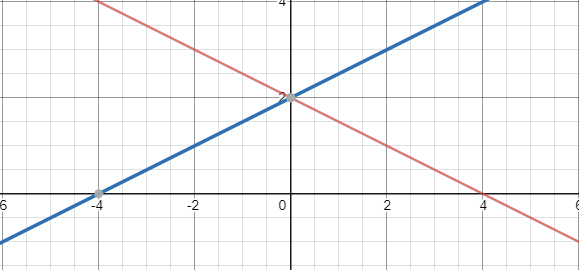
\includegraphics[width=1.0\linewidth]{4-1_a-15b}
consistent and \\independent
\vfill\null
\columnbreak
	\begin{align*}
		&\text{Infinite solutions} \\
		&\begin{bmatrix}
			1 & m & | & h\\
			0 & 0 & | & 0
		\end{bmatrix} 
	\end{align*}
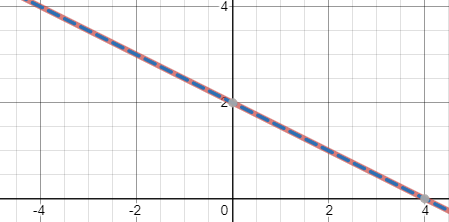
\includegraphics[width=1.0\linewidth]{4-1_a-15c}
consistent and \\dependent
\vfill\null
\columnbreak
	\begin{align*}
		&\text{No solution} \\
		&\begin{bmatrix}
			1 & m & | & h\\
			0 & 0 & | & k
		\end{bmatrix} 
	\end{align*}
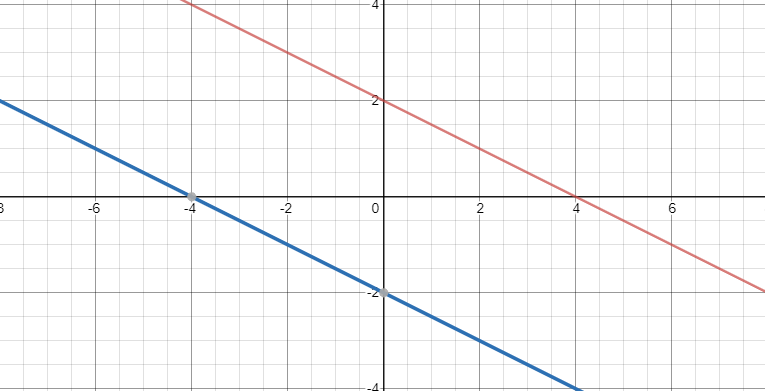
\includegraphics[width=1.0\linewidth]{4-1_a-15}
inconsistent\\
\vfill\null
\end{multicols}



\end{document}
